Loci can be ellipses, but can they be a circle? Let $P$ be an $N=3$ vertex and $P'$ its reflection about the origin. By symmetry, this will ``fall" on the Billiard. Let  $Q_1$ and $Q_2$ be intersections of the tangent to the Billiard at $P'$ with the orbit's Excentral Triangle $T'$. The following remarkable property holds, illustrated in Figure~\ref{fig:cosine_circle_locus}: 

\begin{figure}[H]
\centering
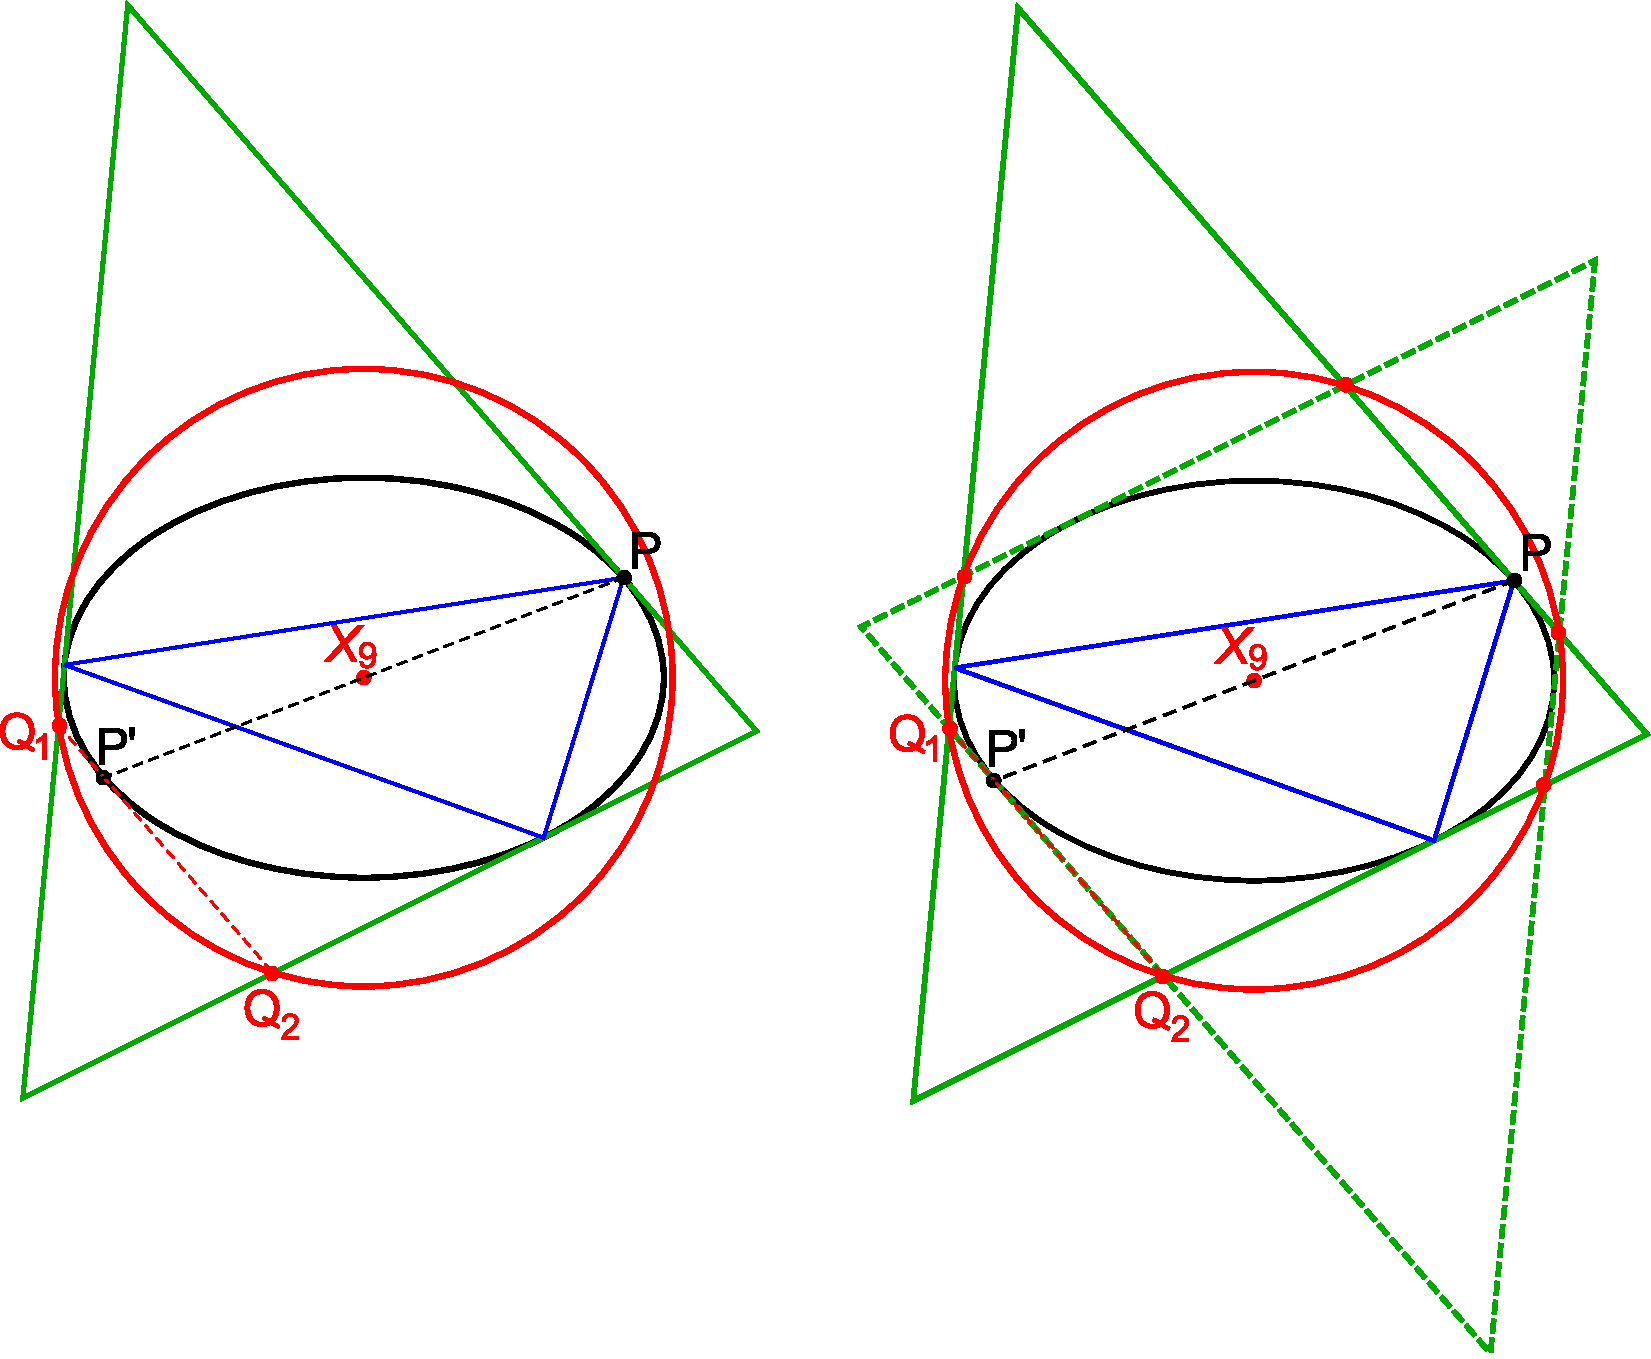
\includegraphics[width=.8\linewidth]{pics/u0110_cosine_circle_locus.pdf}
\caption{\textbf{Left}: Circular Locus of $Q_1$ (or $Q_2$). \textbf{Right}: The Excentral Triangle's six intersections with its reflection about its Symmedian Point (congruent with $X_9$) is a circle. \href{https://youtu.be/CrOSI8d8qDc}{Video 1}, \href{https://youtu.be/hCQIT6_XhaQ}{Video 2} \cite[pl\#16,17]{dsr_math_intell_playlist}}
\label{fig:cosine_circle_locus}
\end{figure}

\begin{theorem}
The locus of $Q_1$ (or $Q_2$) is a circle centered on the Billiard's.
\end{theorem}

The circular locus\footnote{For Triangle enthusiasts, the circular locus is congruent with the {\em Cosine Circle} of the Excentral Triangle, also known as the {\em Second Lemoine Circle}, a kind of {\em Tucker Circle} \cite{mw}. Its center is the Symmedian Point of the Excentral. Since the latter is congruent with the orbit's Mittenpunkt, both radius and center are stationary. No other Tucker Circles for the $N=3$ family have been found to be stationary.} is always external to the Billiard and its radius $r^*$ can be written as a function of the aspect ratio \cite{ronaldo19a}, or even more simply \cite{dominique19,sergei19_private_circles}:

\begin{equation}
r^* = %\frac{\sqrt{3}}{3}\sqrt{2\delta+a^2+1}=
\frac{L}{\frac{r}{R}+4} = \frac{1}{\gamma}\;.
\label{eqn:rstar}
\end{equation}

This surprising phenomenon can be viewed here \cite[pl\#16,17]{dsr_math_intell_playlist}.
